\documentclass{./../div_teaching_slides}

\begin{document}
\title{ECON 340 \\ Economic Research Methods}
\author{Div Bhagia}
\date{Lecture 15: Ordinary Least Squares, Goodness of Fit}

%%%%%%%%%%%% 
\begin{frame}[noframenumbering, plain]
\maketitle
\end{frame}


%%%%%%%%%%%% 
\begin{frame}{Student-Teacher Ratio and Test Scores}
\centering
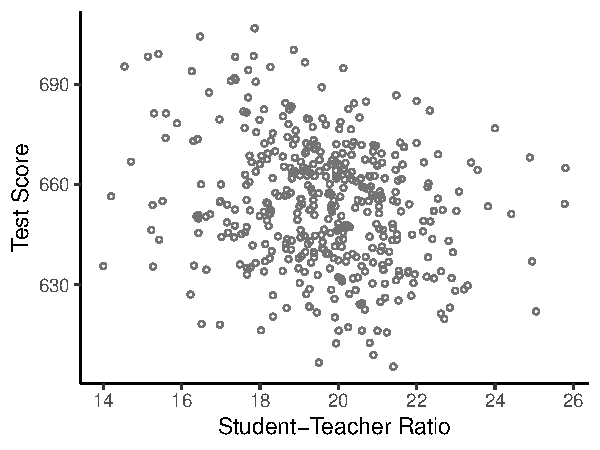
\includegraphics{./../../output/lrm_caschool_scatter1.pdf}
\end{frame}

%%%%%%%%%%%% 
\begin{frame}{Fitting a Line}
\begin{witemize}
  \item We are interested in the relationship between two variables $X$ and $Y$
  \item We start by assuming there is a linear relationship (with some error) between these variables in the population 
 $$ Y = \beta_0 + \beta_1 X + u $$
  \item Fit a linear relationship between these two variables using sample data
\end{witemize}
\end{frame}

%%%%%%%%%%%% 
\begin{frame}{Student-Teacher Ratio and Test Scores}
\centering
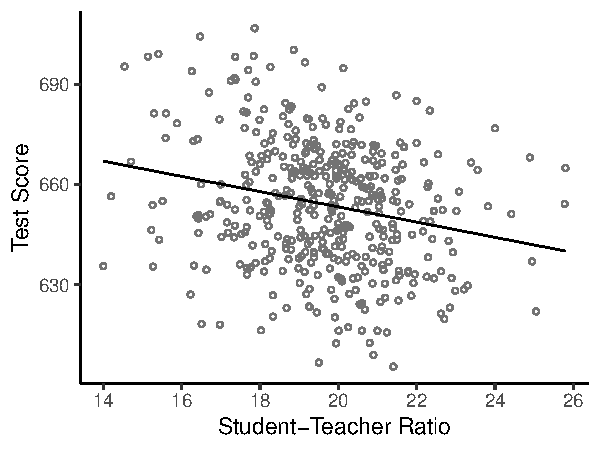
\includegraphics{./../../output/lrm_caschool_scatter2.pdf}
\end{frame}

%%%%%%%%%%%% 
\begin{frame}{Simple Linear Regression Model}
$$ Y = \beta_0 + \beta_1 X + u $$
\vspace{1em}
\begin{witemize}
  \item $Y$: Dependent variable (outcome or response variable)  \item $X$: Independent variable (explanatory variable, regressor)
  \item $\beta_0, \beta_1$: intercept and slope (population parameters)
  \item $u$: mean zero error term, $E(u)=0$
\end{witemize}
\end{frame}

%%%%%%%%%%%% 
\begin{frame}{Which is the best line?}
\centering
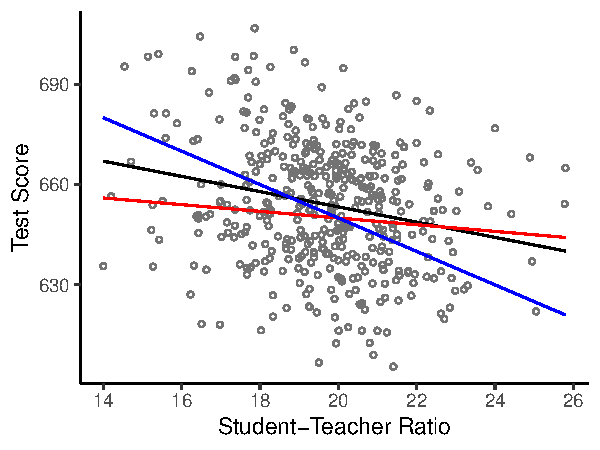
\includegraphics{./../../output/lrm_caschool_bestline.pdf}
\end{frame}


%%%%%%%%%%%% 
\begin{frame}{Ordinary Least Squares (OLS)}
\begin{witemize}
  \item We observe $Y_i$ and $X_i$ for all individuals in our sample.
  \item Find $\hat{\beta_0}$ and $\hat{\beta_1}$ from sample data by minimizing the sum of squared residuals
$$ \min_{b_0, b_1} \sum_{i=1}^n(Y_i - {b_0} - {b_1} X_i)^2$$
\item $\hat{\beta_0}$ and $\hat{\beta_1}$ are called ordinary least squares (OLS) estimators
\end{witemize}
\end{frame}

%%%%%%%%%%%% 
\begin{frame}{Ordinary Least Squares (OLS)}
\begin{columns}[c]
\begin{column}{0.75\textwidth}
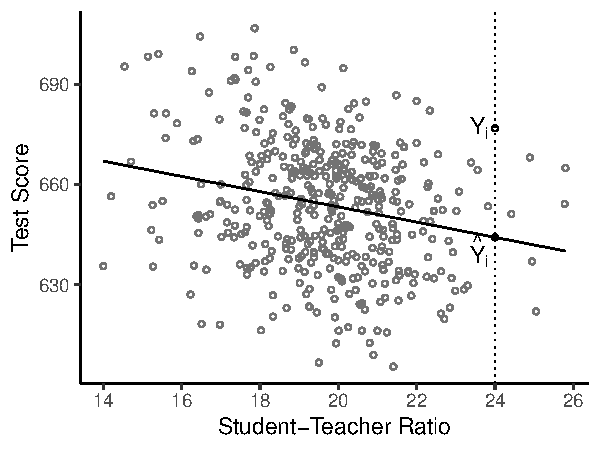
\includegraphics{./../../output/lrm_caschool_ols.pdf}
\end{column}
\begin{column}{0.25\textwidth}
Best line is the one that minimizes: $$\sum_{i=1}^n(Y_i - \hat{Y}_i)^2$$
\vfill
\end{column}
\end{columns}
\end{frame}

%%%%%%%%%%%% 
\begin{frame}{OLS Estimators}
Some calculus reveals:
 $$ \hat{\beta_0} = \bar{Y}-\hat{\beta_1} \bar{X} $$

 $$ \hat{\beta_1} = \frac{ \sum_{i=1}^n(Y_i - \bar{Y})(X_i-\bar{X})}{ \sum_{i=1}^n(X_i - \bar{X})^2 } = \frac{S_{XY}}{S^2_X}$$ 
 
 \vspace{1cm}
 $\rightarrow$ The best-fit line passes through the sample means!
\end{frame}

%%%%%%%%%%%% 
\begin{frame}{OLS line passes through the means}
\centering
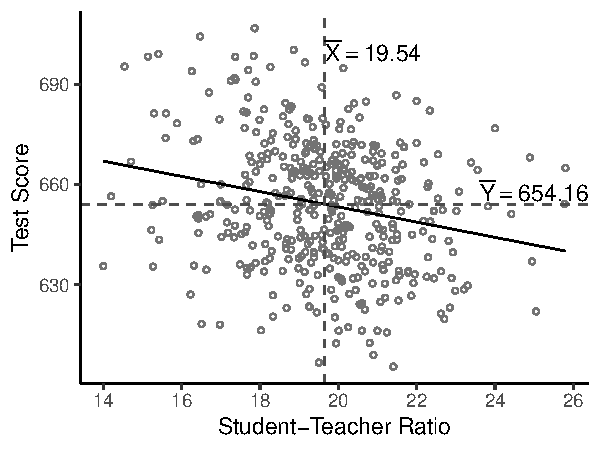
\includegraphics{./../../output/lrm_caschool_means.pdf}
\end{frame}

%%%%%%%%%%%% 
\begin{frame}{Prediction and Residuals}
\vfill
OLS fitted line/predicted values:
$$ \hat{Y_i} = \hat{\beta_0} + \hat{\beta_1} X_i $$
Residuals/prediction error (the one we minimized):
$$ \hat{u}_i = Y_i-\hat{Y}_i $$  
\vfill
\end{frame}

%%%%%%%%%%%% 
\begin{frame}{Prediction and Residuals}
\vfill
For our example, the fitted line:
$$ \hat{testscr} = 698.93 -2.28 \cdot str $$
What is the predicted test score for a school with a student-teacher ratio of 24? \\~\\
What is the prediction error for a school with a student-teacher ratio of 24 and average test score of 677?
\vfill
\end{frame}

%%%%%%%%%%%% 
\begin{frame}{Goodness of Fit: The $R^2$}
\begin{witemize}
  \item $R$-squared measures how well the OLS regression line fits the data
  \item $R$-squared is the percent of sample variation in $Y$ that is explained by $X$ \\~\\
\end{witemize}
Note that:
$$ Y_i = \hat{Y}_i +  \hat{u}_i $$

\vspace{0.5em}
$R^2$ is the ratio of sample variation of $\hat{Y}_i$ to sample variation of $Y_i$
\end{frame}

%%%%%%%%%%%% 
\begin{frame}{Goodness of Fit: The $R^2$}
\begin{itemize}
\item[]   \textit{Total Sum of Squares:} $$ \quad TSS = \sum_{i=1}^n (Y_i-\bar{Y})^2 $$
\item[]  \textit{Explained Sum of Squares:} $$ \quad ESS = \sum_{i=1}^n (\hat{Y}_i-\bar{Y})^2 $$
\item[]   \textit{Residual Sum of Squares:} $$ \quad RSS = \sum_{i=1}^n (Y_i-\hat{Y}_i)^2 =\sum_{i=1}^n \hat{u}_i^2$$
\end{itemize}
\end{frame}


%%%%%%%%%%%% 
\begin{frame}{Goodness of Fit: The $R^2$}
One can show that, $TSS = ESS + RSS$. \\~\\
A measure of goodness of fit: 
$$ R^2 = \frac{ESS}{TSS} = 1-\frac{RSS}{TSS} $$
\end{frame}

%%%%%%%%%%%% 
\begin{frame}{Goodness of Fit: The $R^2$}
\begin{columns}
\begin{column}{0.5\textwidth}
\centering
High $R^2$ \\
	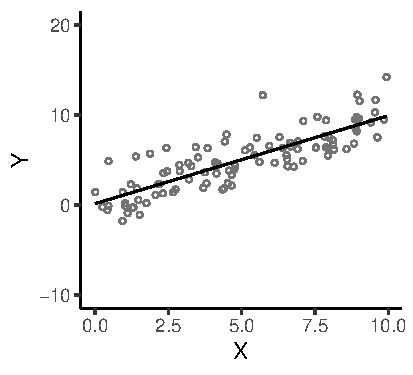
\includegraphics{./../../output/rsquared_high}
\end{column}
\begin{column}{0.5\textwidth}
\centering
Low $R^2$ \\
	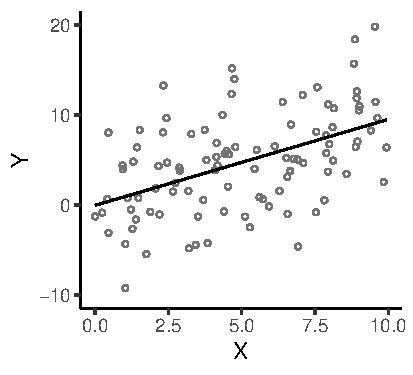
\includegraphics{./../../output/rsquared_low}
\end{column}
\end{columns}

\end{frame}

%%%%%%%%%%%% 
\begin{frame}{Goodness of Fit: The $R^2$}
$$ R^2 = \frac{ESS}{TSS} = 1-\frac{RSS}{TSS} $$

\vspace{1em}
$R^2$ lies between 0 and 1 \\
\begin{witemize}
  \item If $X$ explains no variation in $Y$, $\hat{\beta_1}=0$ and $ \hat{Y_i} = \hat{\beta_0} = \bar{Y}$. In which case, $ESS=0$ and hence $R^2=0$.
  \item On the other hand, if $X$ explains all the variation in $Y$, $\hat{Y}_i=Y_i$ and $RSS=0$. In which case, $R^2=1$.
\end{witemize}
\end{frame}

%%%%%%%%%%%% 
\begin{frame}{How to interpret the coefficients?}
Fitted line:
$$ \hat{testscr} = 698.93 -2.28 \cdot str $$
\begin{witemize}
  \item Intercept: Predicted test score is 698.93 for a school with $str=0$. (Doesn't always make sense!)
  \item Slope: One more student per teacher lowers the predicted test score by 2.28. How? \\ \vspace{0.25em}
   \textit{Alternatively}: Schools in our sample that had one more student per teacher on average had an average test score that was 2.28 points lower.
\end{witemize}
\end{frame}


\end{document}